\documentclass{article}
%Import packages
\usepackage[utf8]{inputenc}
\usepackage{enumitem}
\usepackage{kantlipsum}
\usepackage{xparse}
\usepackage{titlesec}
\usepackage{hyperref}
%Insert mathematical formulae
\usepackage{amsmath}
%Change interlinear space
\usepackage{setspace}
\usepackage{pgfgantt}
\usepackage{float}
\usepackage{graphicx}
\usepackage[table,xcdraw]{xcolor}
\graphicspath{ {imagenes/} }
%Commands
\usepackage{geometry}
 \geometry{
 a4paper,
 total={170mm,257mm},
 left=35mm,
 right=25mm,
 top=20mm,
 }


%Command to add comments in the document without being displayed in the output
\newcommand{\comment}[1]{}

%Rename references section
\renewcommand{\refname}{Bibliografía}

 %Change interlinear spacing

%Allow extra subsection level

\titleclass{\subsubsubsection}{straight}[\subsection]

\newcounter{subsubsubsection}
\renewcommand\thesubsubsubsection{\thesubsubsection.\arabic{subsubsubsection}}
\renewcommand\theparagraph{\thesubsubsubsection.\arabic{paragraph}} % optional; useful if paragraphs are to be numbered

\titleformat{\subsubsubsection}
  {\normalfont\normalsize\bfseries}{\thesubsubsubsection}{1em}{}
\titlespacing*{\subsubsubsection}
{0pt}{3.25ex plus 1ex minus .2ex}{1.5ex plus .2ex}

\makeatletter
\renewcommand\paragraph{\@startsection{paragraph}{5}{\z@}%
  {3.25ex \@plus1ex \@minus.2ex}%
  {-1em}%
  {\normalfont\normalsize\bfseries}}
\renewcommand\subparagraph{\@startsection{subparagraph}{6}{\parindent}%
  {3.25ex \@plus1ex \@minus .2ex}%
  {-1em}%
  {\normalfont\normalsize\bfseries}}
\def\toclevel@subsubsubsection{4}
\def\toclevel@paragraph{5}
\def\toclevel@paragraph{6}
\def\l@subsubsubsection{\@dottedtocline{4}{7em}{4em}}
\def\l@paragraph{\@dottedtocline{5}{10em}{5em}}
\def\l@subparagraph{\@dottedtocline{6}{14em}{6em}}
\makeatother

\setcounter{secnumdepth}{4}
\setcounter{tocdepth}{4}




\begin{document}
\section{Resultados obtenidos}
\paragraph{}
En esta sección se van a detallar las pruebas realizadas así como los resultados obtenidos con su correspondiente interpretación. La tendencia de estos resultados debería ser la misma independientemente de las características del hardware y del sistema operativo utilizado , sin embargo los resultados absolutos varían según estos. Por ello, será necesario especificar el hardware utilizado para dichas pruebas.

\paragraph{}
Todas las pruebas a las que se va a mentar en esta sección son pruebas de eficiencia de los distintos planificadores con las distintas versiones de los problemas. No se ha realizado como tal ninguna prueba funcional a los scripts ya que resulta más fiable y requiere menos tiempo verificar que el resultado de alguna prueba aleatoria de su ejecución coincide con la ejecución manual que diseñar pruebas funcionales que verifiquen lo que ya se ha hecho a mano.

\subsection{Especificaciones del terminal utilizado}
\paragraph{}
Como ya se ha comentado, el hardware y el sistema operativo utilizado influyen en los resultados obtenidos en las pruebas de eficiencia realizadas. Por este motivo, se incluye a continuación las características que pueden influir en estos resultados (otros elementos como los periféricos no son incluídos al no tener ningún efecto sobre los resultados obtenidos).

\begin{itemize}
    \item Tipo de dispositivo: ordenador de sobremesa
    \item Modelo: Hewlett Packard 550-244NS A\footnote{https://support.hp.com/es-es/document/c05045080}
    \item Procesador: AMD A10 8750 
    \item Frecuencia: 3.6GHz
    \item Memoria RAM: 16GB
    \item Sistema operativo: Debian 9
\end{itemize}


\subsection{Pruebas realizadas}
\paragraph{}
Las pruebas que se han realizado tenían como fin demostrar algo que la revisión del estado del arte y que intuitivamente se conocía: que tanto el tiempo de búsqueda de un planificador como la calidad de la solución de un mismo problema podía variar con la modificación de la representación del dominio y/o del problema. El software utilizado de otros investigadores que ha sido utilizado para estas pruebas como se explicó en la sección de la solución propuesta tiene sus limitaciones y no es capaz de encontrar siempre las mejores modificaciones que sí son posibles encontrar a mano. Esto es algo que intuitivamente era de esperar que en esta sección se intentará cuantificar el coste que supone la automatización de estas modificaciones.

\paragraph{}
Las pruebas han sido realizadas con dos planificadores, Metric-FF y LPG-td (el funcionamiento de ambos planificadores puede encontrarse en la sección de la solución propuesta). Inicialmente también se encontraba el planificador FastDownward ejecutado con la métrica de Lama2011. Sin embargo, este planificador ha sido descartado y sus resultados no se han incluido en esta sección ya que el planificador no fue capaz de resolver un solo problema de ninguno de los problemas de las distintas versiones introducidas como entradas, mientras que los 20 problemas de alguna de esas versiones eran resueltos en su totalidad por ambos planificadores en menos de 10 minutos.

\paragraph{}
Por tanto, podría haberse aumentado el número de planificadores utilizados para la sección de pruebas. Sin embargo, teniendo en cuenta que una estimación muy benévola de la sección de planificación del proyecto se estimaba el número de horas de ejecución de las pruebas funcionales en 139 horas de ejecución, la inclusión de pruebas con nuevos planificadores implicarían un gasto de tiempo considerable. Por tanto, si se hubiese dispuesto de más tiempo, estas pruebas posteriores se cree que podrían haber servido para entender la relación de las modificaciones realizadas con un entorno más amplio de planificadores para así quizá poder incluso a poder sacar conclusiones apriorísticas sobre el tipo de modificaciones que pueden beneficiar a un tipo concreto de planificador. Esto por falta de tiempo no ha podido ser realizado por lo que se encuentra entre las líneas de trabajo por las que se podría continuar este trabajo.

\paragraph{}
Existe también otra altertiva que es realizar las pruebas exclusivamente con un único planificador. Esta opción podría hacer que se extrajesen conclusiones equivocadas o muy limitadas respecto a las modificaciones realizadas en los dominios, puesto que la mejora en la planificación que se puede obtener con dichas modificaciones depende del planificador y de la heurística que éste utilice.

\paragraph{}
Los parámetros de ejecución utilizados para estos planificadores son:

\begin{itemize}
    \item Metric-FF: -s 0 (FF estándar: EHC+H y BFS).
    \item LPG-td: -n 1 (genera únicamente una solución).
\end{itemize}

\paragraph{}
El tiempo de ejecución máximo para la resolución de cada problema es de 30 minutos tal y como se efectúa en las competiciones de la IPC.

\paragraph{}
Respecto al coste de las acciones, la ejecución de las acciones de todas las versiones tienen coste 1 salvo en el caso de los dominios con macrooperadores, en cuyo caso los macrooperadores tendrán el coste del número de operadores del dominio original que estén sustituyendo.

\subsection{Resultados obtenidos}

\subsubsection{Comparación de dominios 01 y 03}
\paragraph{}
En esta sección, se van a comparar los resultados obtenidos al ejecutar las siguientes versiones de los problemas que se han generado utilizando macrooperadores (es decir, la versión 01 y 03 de los problemas realizados a mano).

\paragraph{}
Como ya se comentó en la sección de la solución propuesta, en esta sección no se van a incluir los tiempos de ejecución de la versión obtenida mediante las modificaciones de PTT puesto que este software no fue capaz de realizar una sola modificación del dominio original, por lo que todos los resultados funcionales serían idénticos a los del dominio original puesto que es el mismo.

\pagebreak

\begin{figure}[!htb]
   \begin{minipage}{0.48\textwidth}
     \centering
     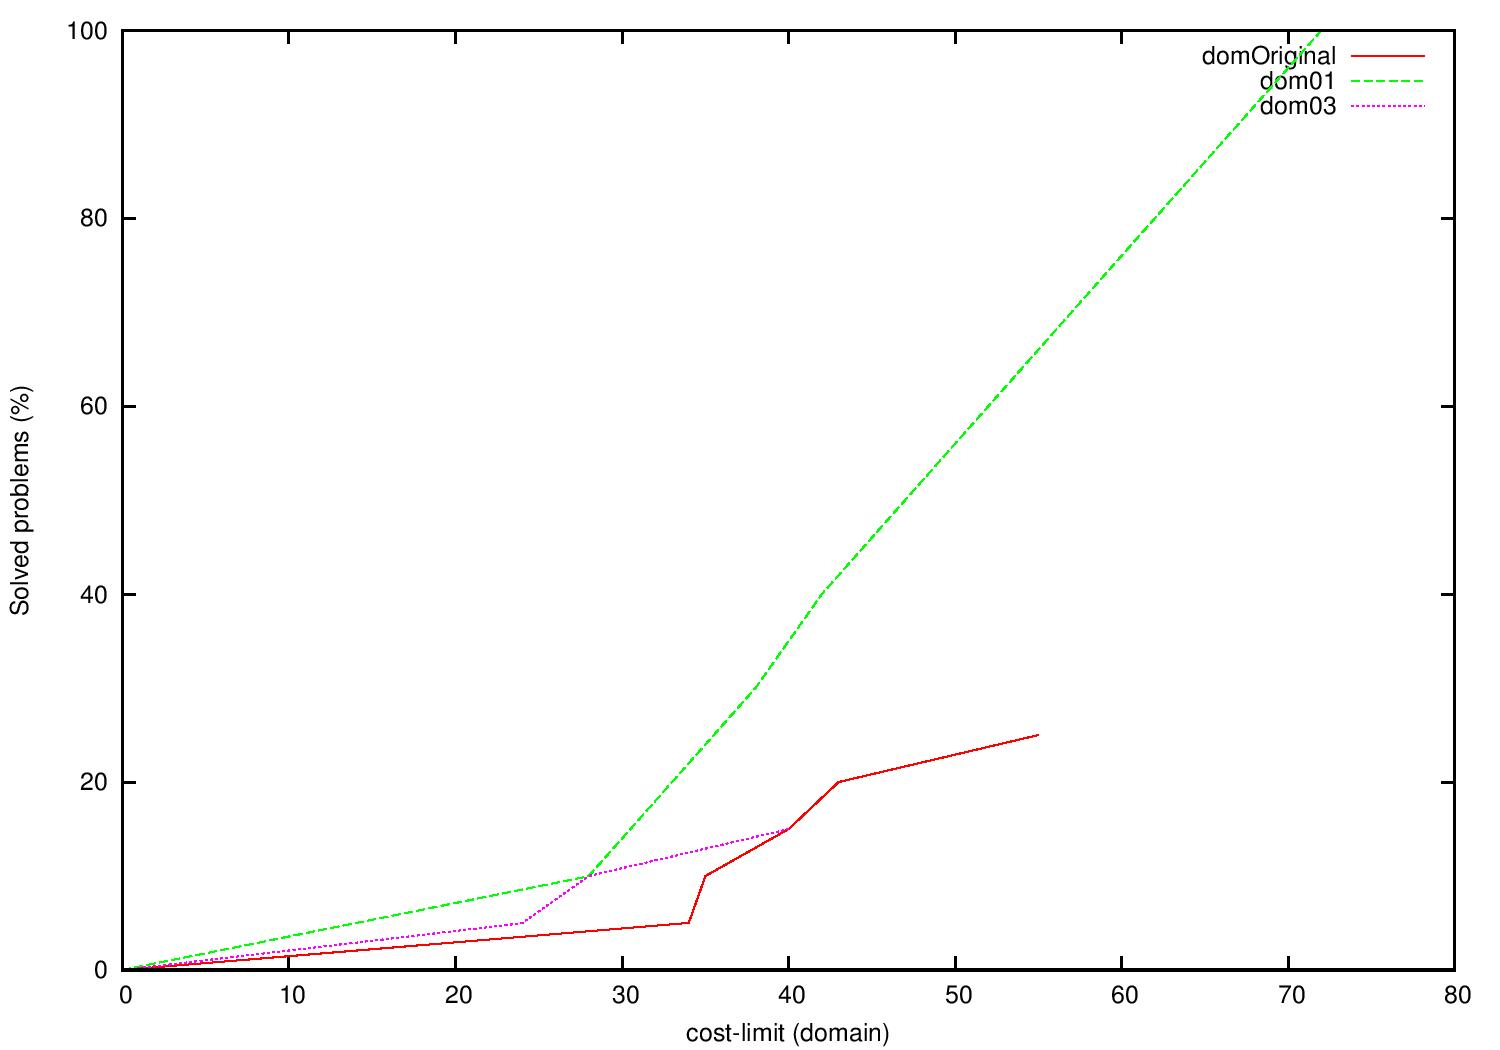
\includegraphics[width=6cm, height=6cm]{mff-or-01-03-cost}
    \caption{MFF-original-01-03-coste}
   \end{minipage}\hfill
   \begin {minipage}{0.48\textwidth}
     \centering
     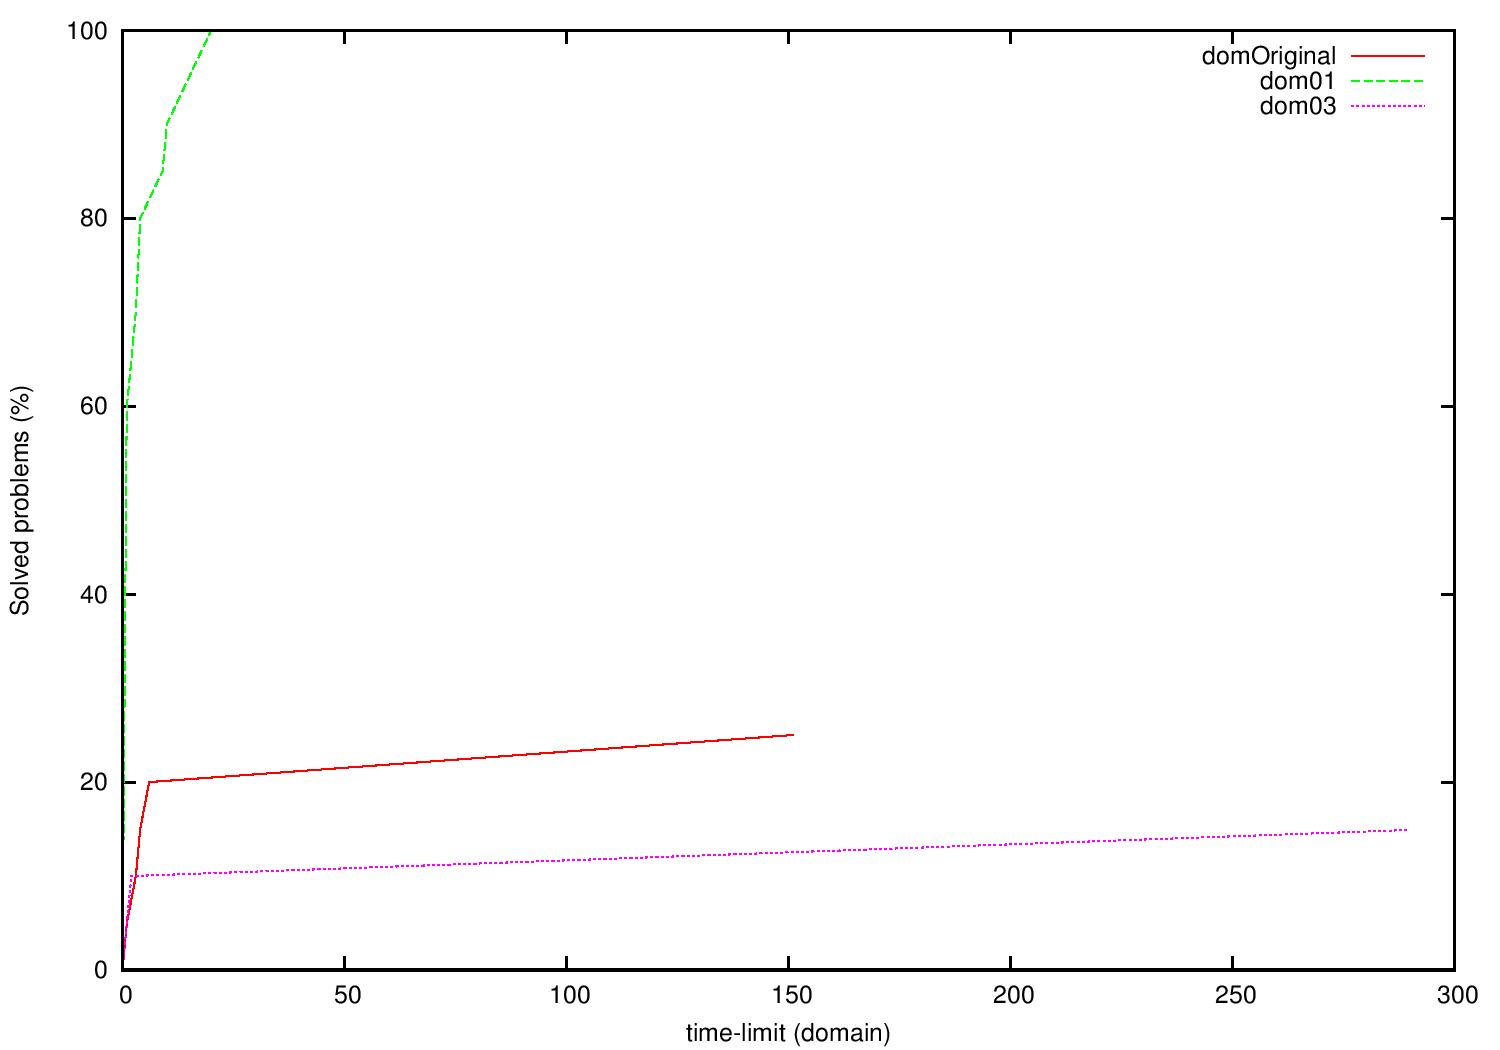
\includegraphics[width=6cm, height=6cm]{mff-or-01-03-time}
    \caption{MFF-original-01-03-tiempo}
   \end{minipage}
\end{figure}

\begin{figure}[!htb]
   \begin{minipage}{0.48\textwidth}
     \centering
     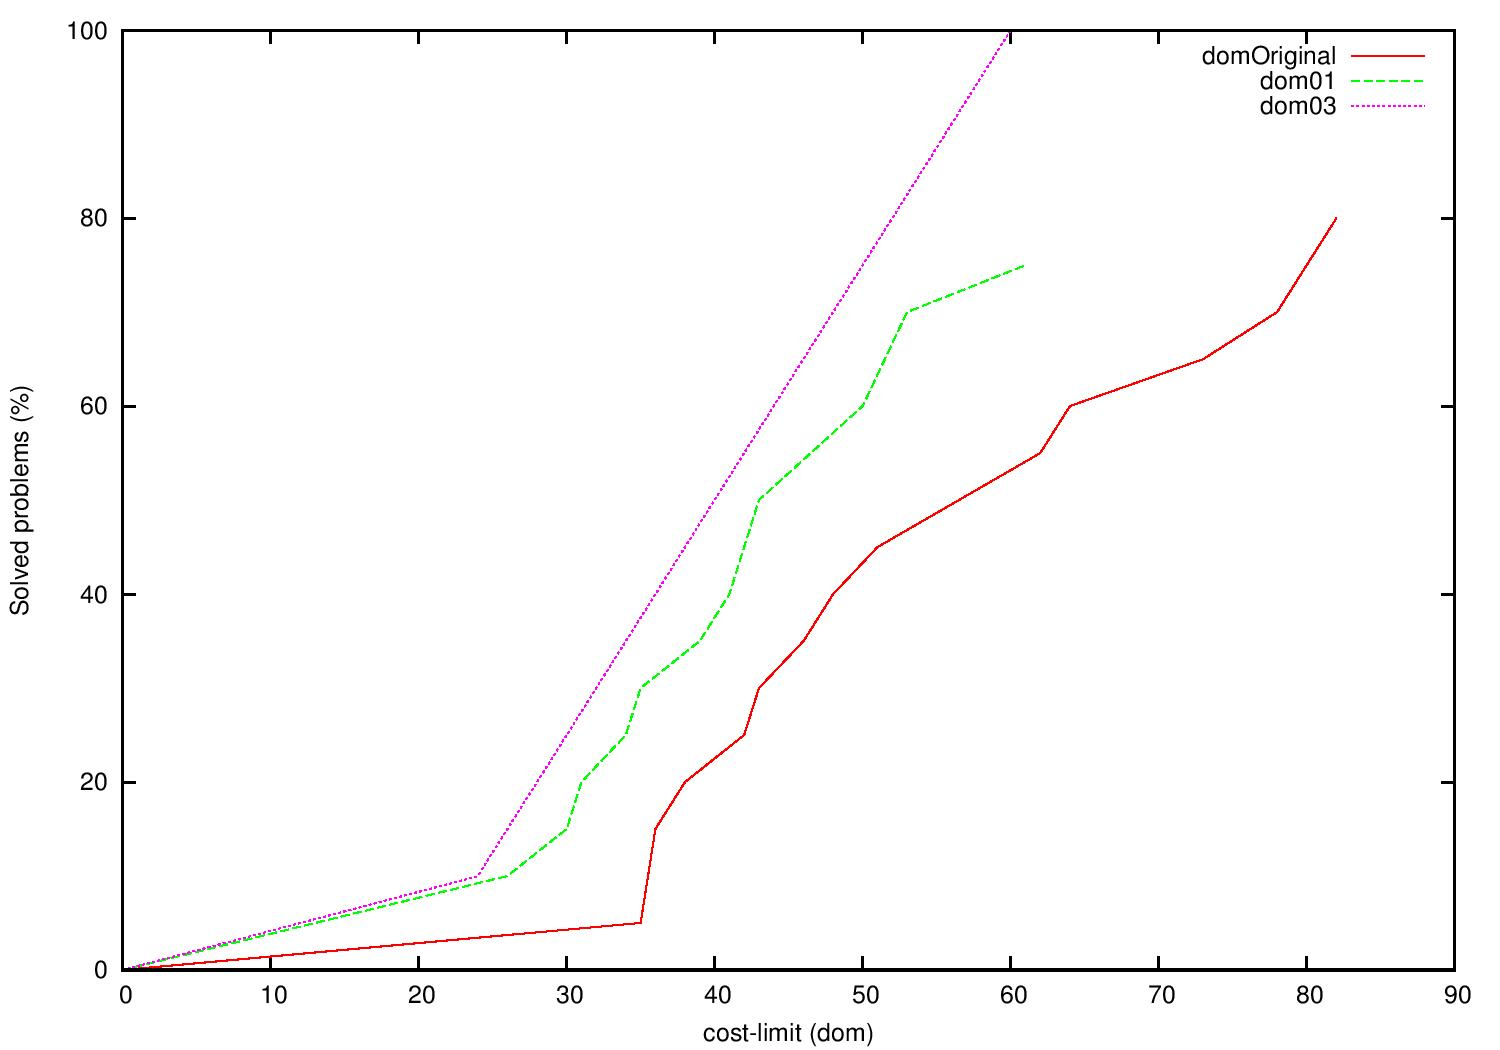
\includegraphics[width=6cm, height=6cm]{lpg-or-01-03-cost}
    \caption{LPG-original-01-03-coste}
   \end{minipage}\hfill
   \begin {minipage}{0.48\textwidth}
     \centering
     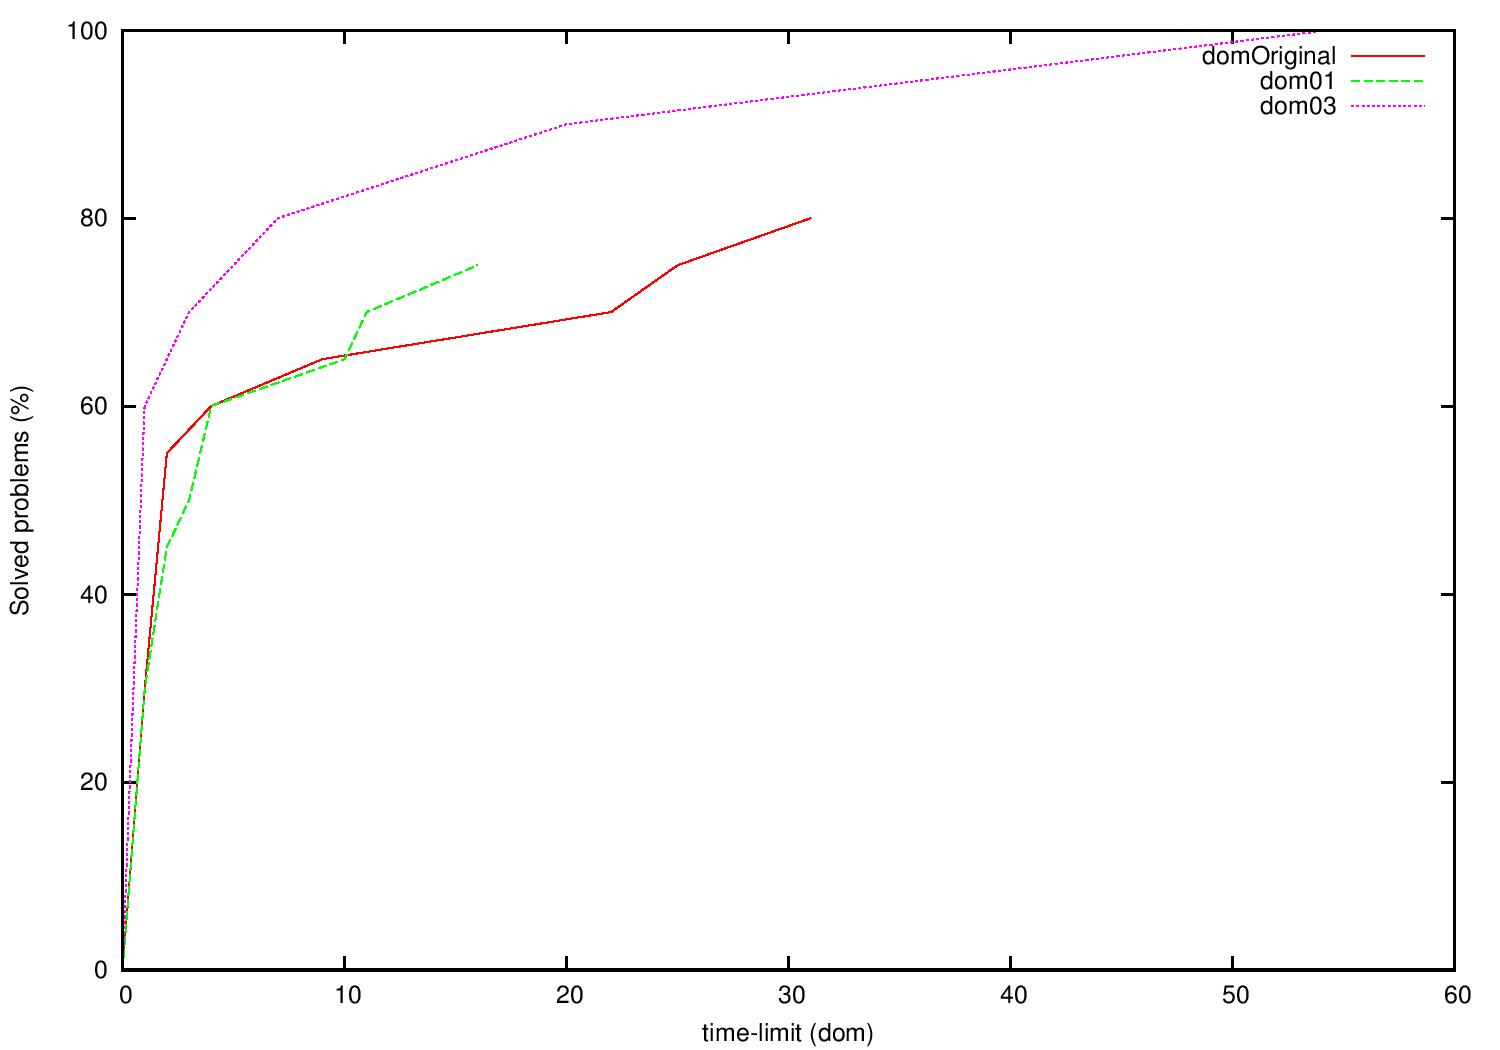
\includegraphics[width=6cm, height=6cm]{lpg-or-01-03-time}
    \caption{LPG-original-01-03-tiempo}
   \end{minipage}
\end{figure}

\paragraph{}
En los resultados obtenidos con MFF se puede ver que el coste para resolver los mismos problemas es mayor en la versión 01 que tanto en la versión original como en la versión 03. De hecho, la que tiene un menor coste de las tres es la versión original. Por otro lado, en la versión 01 consigue resolver todos los problemas, a diferencia de lo que ocurre en la versión 03 que resuelve además menos problemas que la versión original. A esto hay que añadir que el tiempo de ejecución para la resolución de los problemas es muy inferior en el caso de la versión 01 y es superior en el caso de la versión 03.

\paragraph{}
La interpretación que se hace de estos resultados es que mientras que en el primero la \textit{utilidad} del macrooperador está ajustada para que contrarreste los efectos negativos que produce por ejemplo un mayor coste para obtener la solución, este no es el caso de la versión 03. La versión 03 se ha hecho explícitamente para mostrar el resultado que se obtiene cuando se genera un macrooperador con una interfaz demasiado grande que hace que la utilidad de dicho macrooperador sea negativa, como se puede ver en los resultados. Por otro lado, en la versión 01 se obtiene la ventaja de que al unir dos operadores que frecuentemente se suelen suceder (el operador de movimiento del carrito y el operador de de servir el sándwich), como se han retirado los operadores iniciales, esto reduce el factor de ramificación del árbol de búsqueda pero a su vez implica obtener soluciones más costosas puesto que si por ejemplo dos niños están en la misma posición, en lugar de realizar la solución óptima que sería cargar los dos sándwiches en una bandeja (2), mover la bandeja a la localización de los niños (1) y servirles (2), lo que supone un gasto de 5 unidades, con esta solución habría que cargar un sándwich en la bandeja (1), mover el carro y servir a un niño (2), mover el carro de vuelta a la cocina (1), cargar un sándwich (1) en la bandeja, mover la bandeja y servir el sándwich (2), lo que supone un gasto de 7 unidades, dos más que en la solución original.

\paragraph{}
Respecto a los resultados obtenidos con LPG, con la versión 03 se consiguen resolver todos los problemas en el menor de los tiempos posibles de las tres versiones. En este caso, la versión 01 resuelve menos problemas que en la versión original pero los problemas que resuelve lo hace en menos tiempo que en la versión original.

\subsubsection{Comparación del dominio02}

\paragraph{}
En esta sección, se va a comparar la pequeña modificación realizada en uno de los operadores del dominio original respecto a la versión original. La modificación únicamente deja de etiquetar como que tuviesen gluten los sándwiches generados con dos componentes sin gluten que aparezcan como entrada del operador \textit{make\_sandwich}. Este es un caso muy concreto en el que como se comentó en la sección de la solución propuesta, debería reducir el tiempo de búsqueda para encontrar la solución pero muy ligeramente, puesto que como se ha dicho no es un caso genérico, sino uno muy concreto para una única operación.

\pagebreak

\begin{figure}[!htb]
   \begin{minipage}{0.48\textwidth}
     \centering
     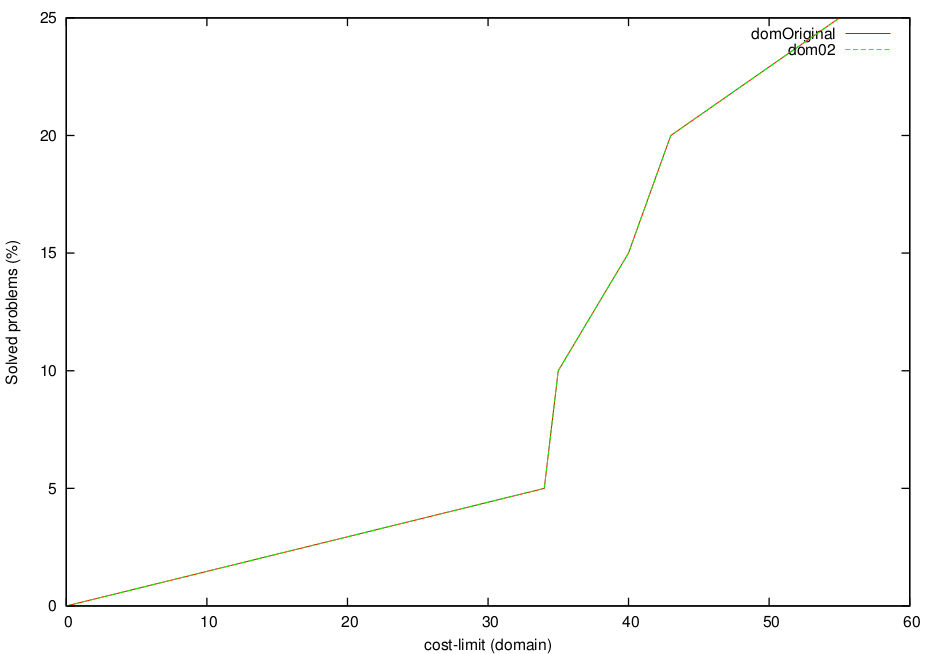
\includegraphics[width=6cm, height=6cm]{mff-or-02-cost}
    \caption{MFF-original-02-coste}
   \end{minipage}\hfill
   \begin {minipage}{0.48\textwidth}
     \centering
     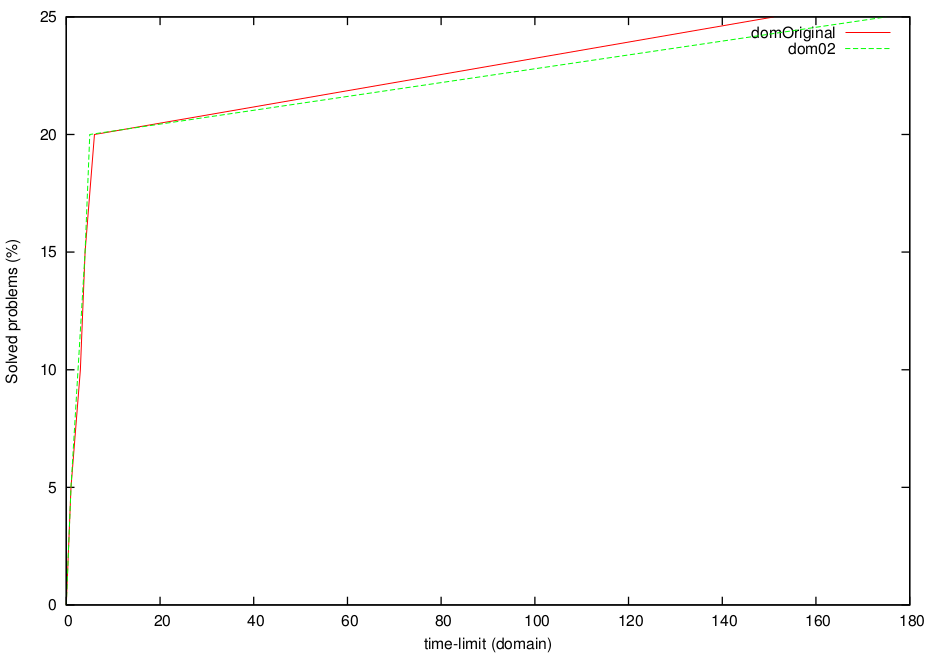
\includegraphics[width=6cm, height=6cm]{mff-or-02-time}
    \caption{MFF-original-02-tiempo}
   \end{minipage}
\end{figure}

\begin{figure}[!htb]
   \begin{minipage}{0.48\textwidth}
     \centering
     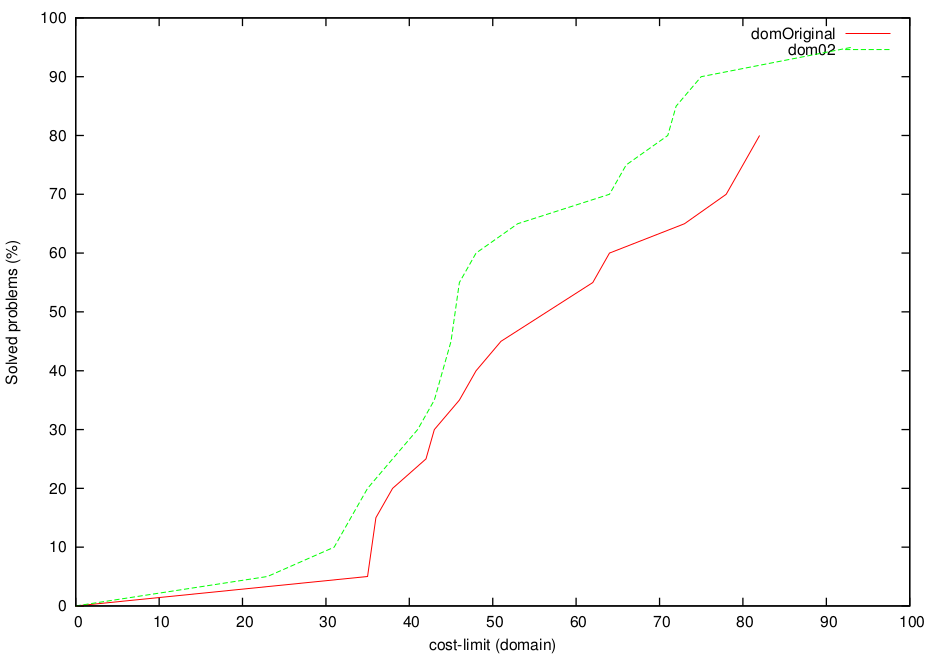
\includegraphics[width=6cm, height=6cm]{lpg-or-02-cost}
    \caption{LPG-original-02-coste}
   \end{minipage}\hfill
   \begin {minipage}{0.48\textwidth}
     \centering
     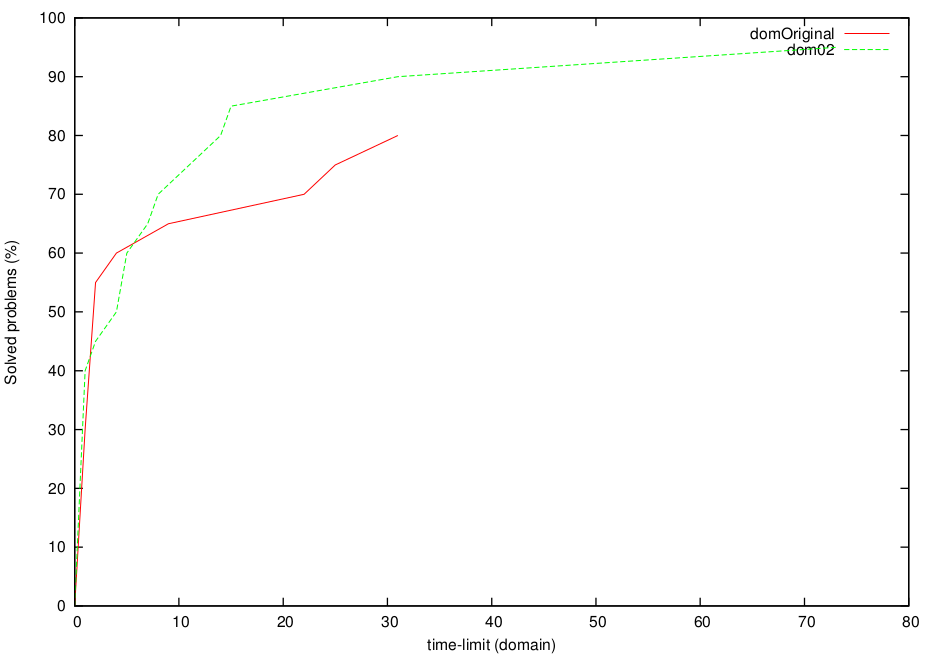
\includegraphics[width=6cm, height=6cm]{lpg-or-02-time}
    \caption{LPG-original-02-tiempo}
   \end{minipage}
\end{figure}

\paragraph{}
Como se puede ver en las gráficas obtenidas en MFF, esta versión reduce ligeramente el tiempo de búsqueda y esta mejora se va acrecentando a medida que aumenta el tamaño de los problemas. Esto es debido a que con el aumento del tamaño de los mismos, aumenta la probabilidad de que ocurra el caso particular en el que el segundo dominio provoca una reducción del tiempo de búsqueda. Respecto al coste, se puede ver que es idéntico en ambos casos, puesto que realmente lo que se consigue con esta nueva versión es podar del árbol de búsqueda soluciones duplicadas (que podrían ser obtenidas mediante el otro operador de crear sándwiches con gluten) o erróneas, por lo que la solución final encontrada por ambas versiones es muy probable que acabe siendo la misma.

\paragraph{}
Las gráficas obtenidas con LPG-td son más difíciles de interpretar y no siguen el mismo patrón que en Metric-FF. En estas, con la nueva versión sí se producen importantes modificaciones tanto en el tiempo consumido como en el coste de las soluciones obtenidas. Respecto al tiempo consumido, con la versión original se resuelven 3 problemas menos y los problemas resueltos requieren de más tiempo. Por otro lado, el coste de resolución de estos problemas es también superior en la versión original.

\subsubsection{Comparación del dominio09 y dominio11}
\paragraph{}
En estas versiones, se realiza exclusivamente la modificación de los predicados aumentando o disminuyendo su tamaño de interfaz. En el caso de la versión 09, se aumenta dicho tamaño al juntar los predicados de \textit{allergic\_gluten} y \textit{not\_allergic\_gluten} con el predicado \textit{waiting}, ya que en ambas partes de los predicados originales se refiere a la misma variable \textit{child}. En la versión 11, se sustituye el predicado de negación \textit{not\_allergic\_gluten} por la negación del predicado \textit{allergic\_gluten}m es decir, \textit{(not(allergic\_gluten))}.

\pagebreak

\begin{figure}[!htb]
   \begin{minipage}{0.48\textwidth}
     \centering
     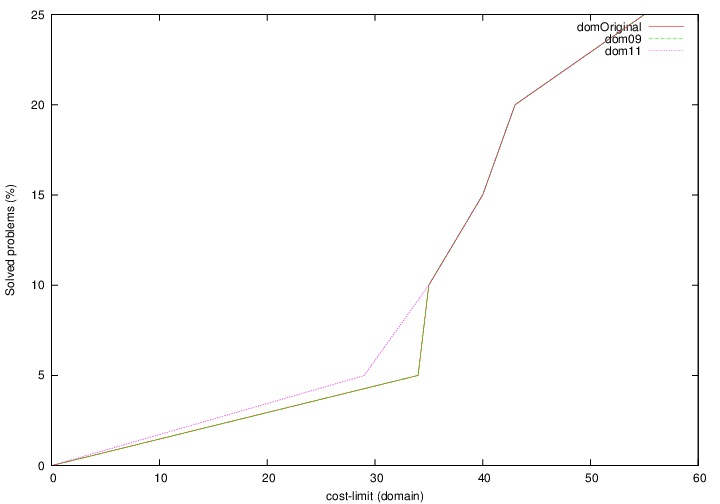
\includegraphics[width=6cm, height=6cm]{mff-or-09-11-cost}
    \caption{MFF-or-09-11-coste}
   \end{minipage}\hfill
   \begin {minipage}{0.48\textwidth}
     \centering
     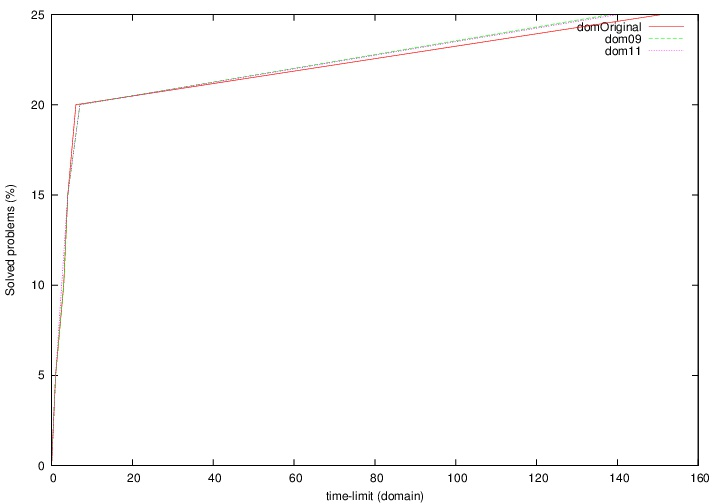
\includegraphics[width=6cm, height=6cm]{mff-or-09-11-time}
    \caption{MFF-or-09-11-tiempo}
   \end{minipage}
\end{figure}

\begin{figure}[!htb]
   \begin{minipage}{0.48\textwidth}
     \centering
     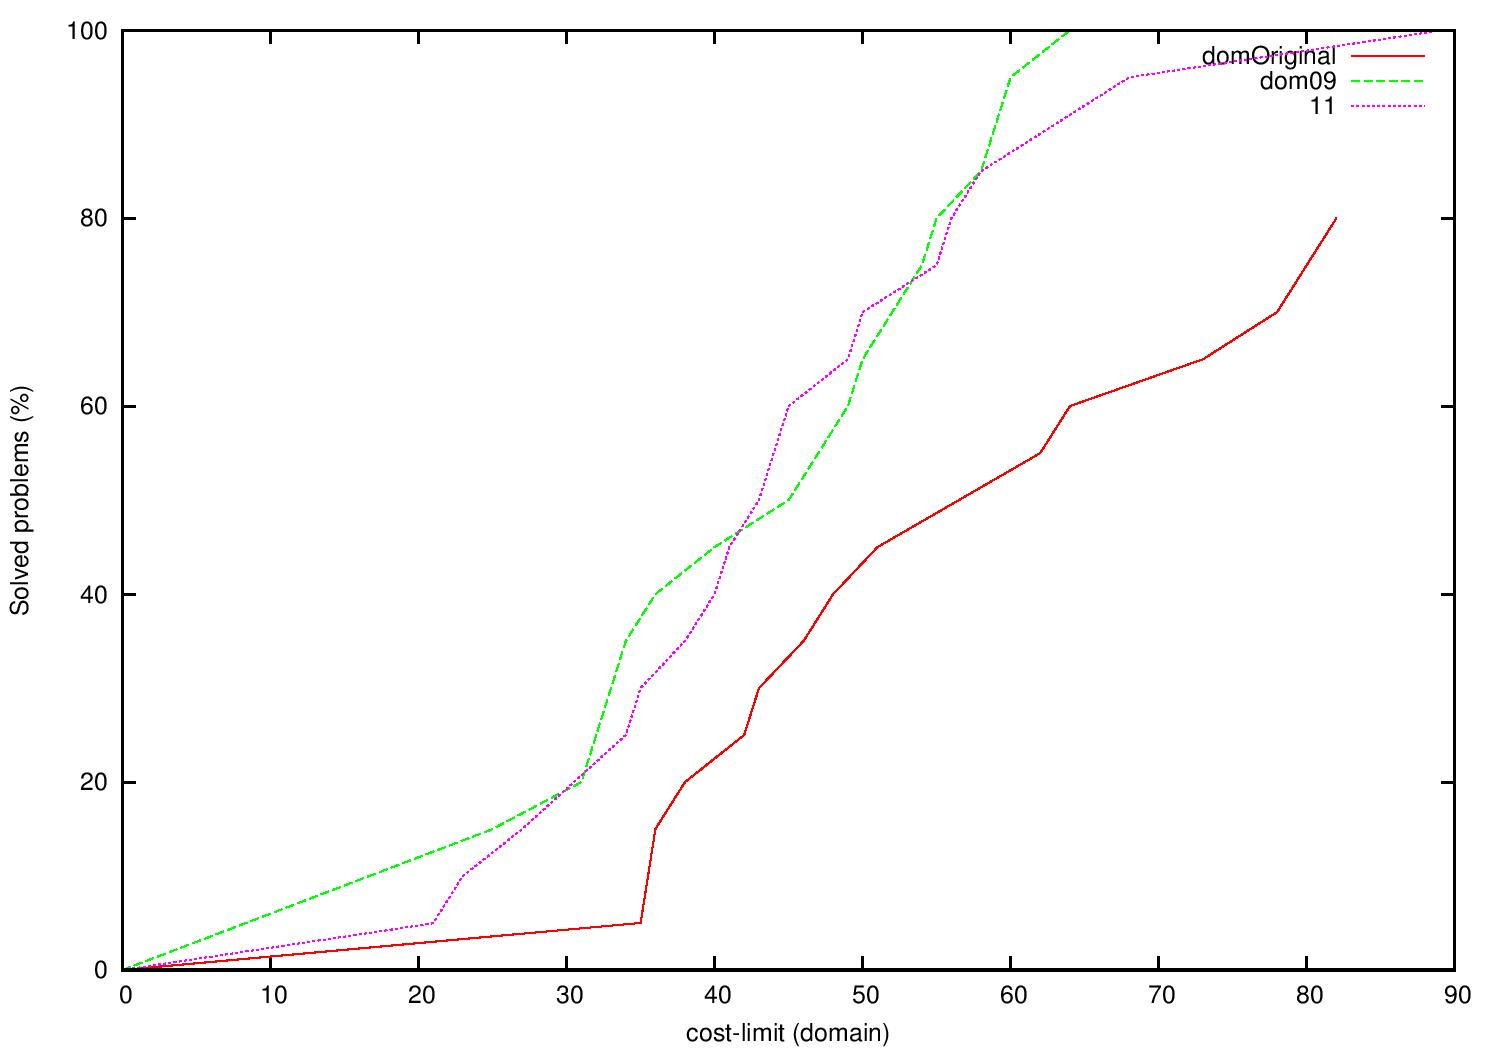
\includegraphics[width=6cm, height=6cm]{lpg-or-09-11-cost}
    \caption{LPG-or-09-11-coste}
   \end{minipage}\hfill
   \begin {minipage}{0.48\textwidth}
     \centering
     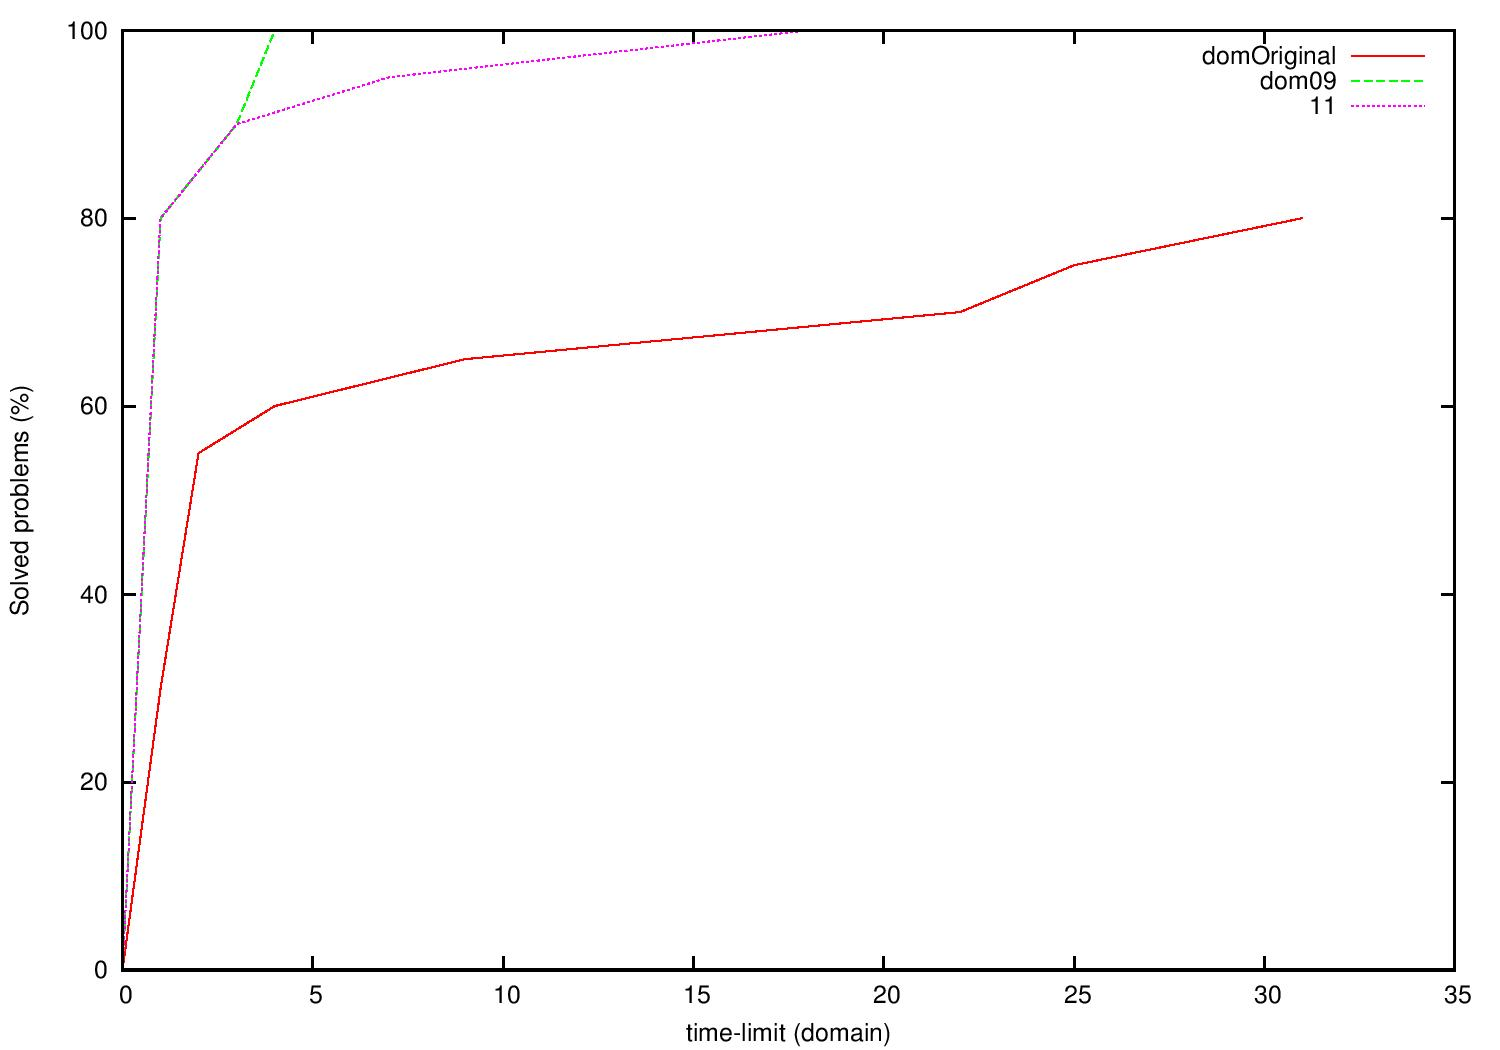
\includegraphics[width=6cm, height=6cm]{lpg-or-09-11-time}
    \caption{LPG-or-09-11-tiempo}
   \end{minipage}
\end{figure}

\paragraph{}
Respecto a los resultados obtenidos con MFF, con la versión 09 se obtienen soluciones con exactamente el mismo coste que en la versión original a diferencia de la versión 11, con la que se obtienen problemas con menor coste hasta llegar a problemas con una complejidad en la que convergen los costes de las tres versiones. Respecto a los problemas y el tiempo de resolución, todos convergen en la resolución de el 25\% de los problemas pero con una ligera reducción de tiempo de búsqueda en las dos versiones realizadas a mano. Al haberse realizado modificaciones pequeñas de los predicados, no se esperaban grandes cambios en la calidad y los tiempos de ejecución, por lo que era previsible que estos resultados fueran cercanos a los obtenidos con la versión original.

\paragraph{}
En relación a los resultados obtenidos con LPG, estos son mucho más impredecibles y difíciles de interpretar. Ambas versiones consiguen aumentar el porcentaje de problemas resueltos de en torno al 80\% al 100\%. El coste de dichas resoluciones es inferior que en el caso original y dependiendo del tramo es mayor o menor el coste entre ambas versiones. Finalmente, respecto al tiempo de ejecución, los menores tiempos se obtienen con la versión 09, aunque con la versión 11 también se reducen los tiempos de ejecución respecto a la versión original.



\pagebreak

\begin{figure}[!htb]
   \begin{minipage}{0.48\textwidth}
     \centering
     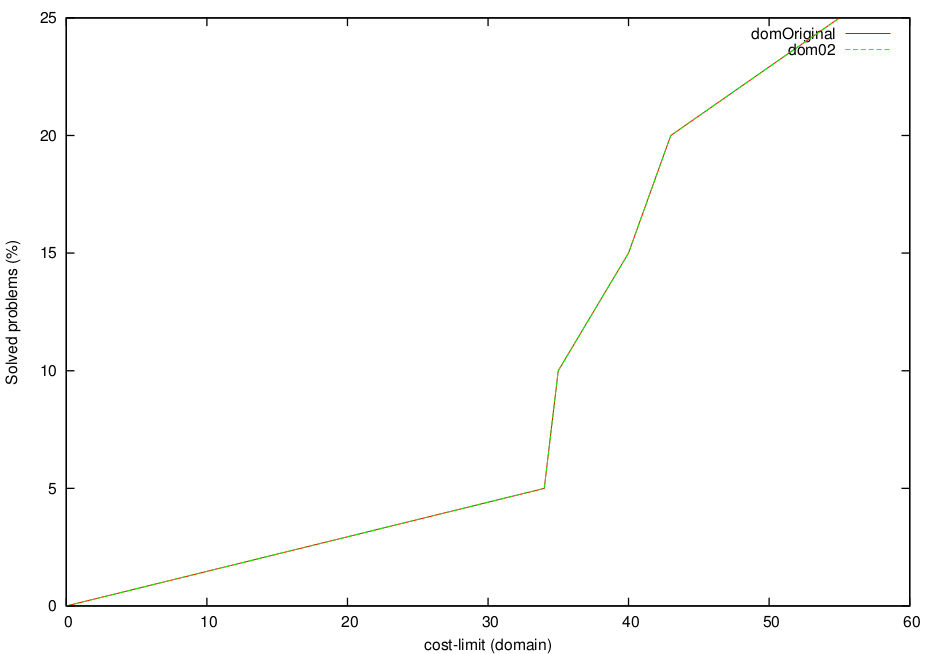
\includegraphics[width=6cm, height=6cm]{mff-or-02-cost}
    \caption{MFF-original-02-coste}
   \end{minipage}\hfill
   \begin {minipage}{0.48\textwidth}
     \centering
     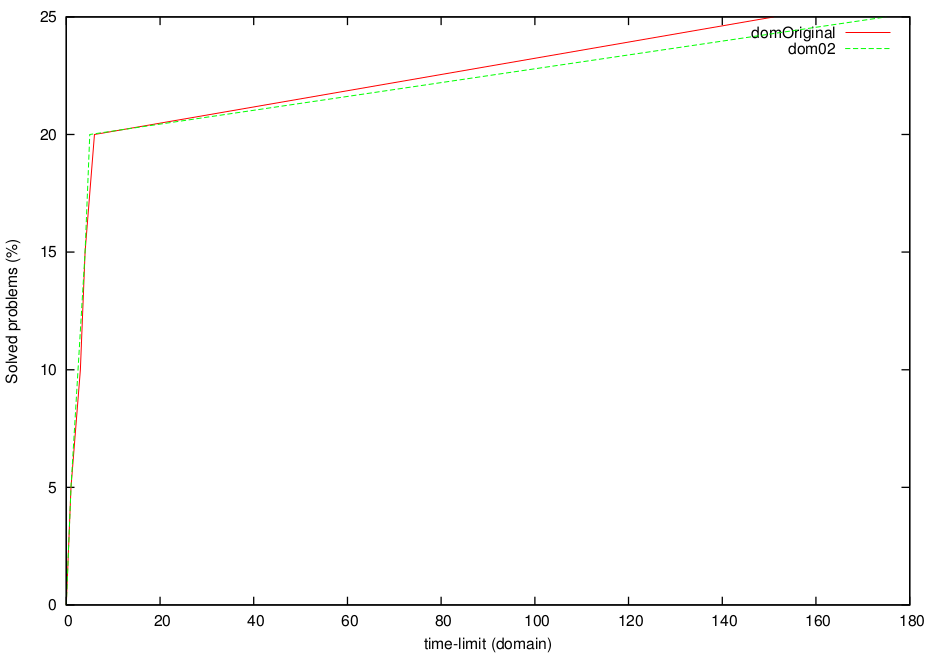
\includegraphics[width=6cm, height=6cm]{mff-or-02-time}
    \caption{MFF-original-02-tiempo}
   \end{minipage}
\end{figure}

\begin{figure}[!htb]
   \begin{minipage}{0.48\textwidth}
     \centering
     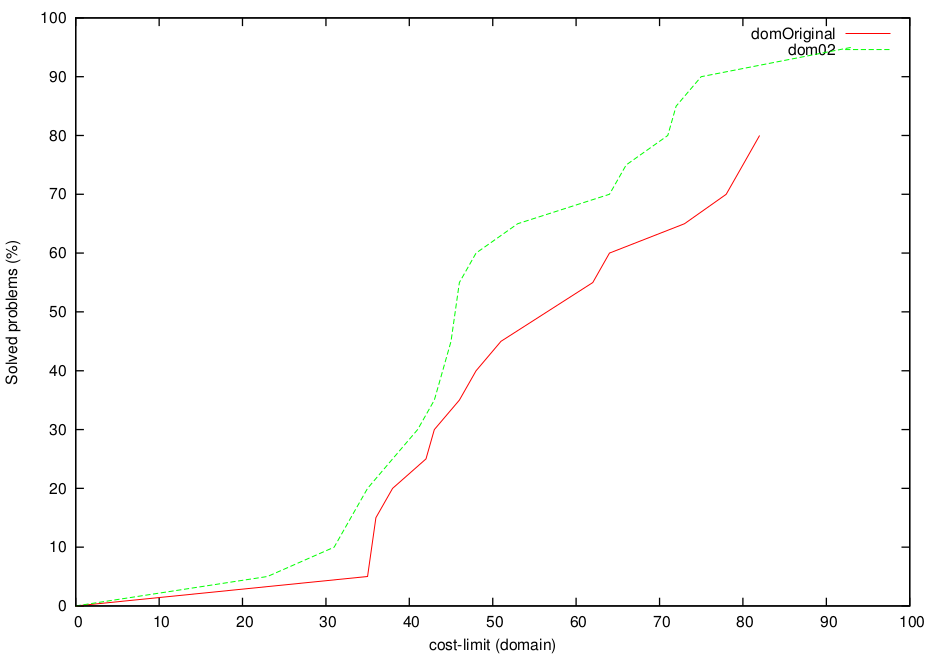
\includegraphics[width=6cm, height=6cm]{lpg-or-02-cost}
    \caption{LPG-original-02-coste}
   \end{minipage}\hfill
   \begin {minipage}{0.48\textwidth}
     \centering
     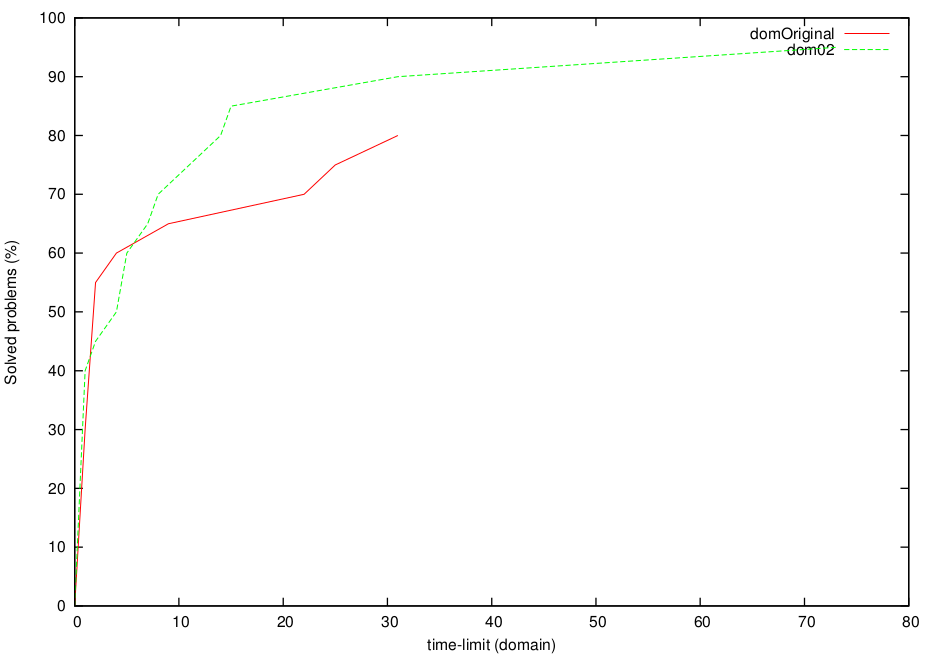
\includegraphics[width=6cm, height=6cm]{lpg-or-02-time}
    \caption{LPG-original-02-tiempo}
   \end{minipage}
\end{figure}

\subsubsection{Comparación de los dominios numéricos}
\paragraph{}
En esta sección, se van a comparar tanto los dominios numéricos realizados a mano como los dominios numéricos obtenidos obtenidos mediante software independiente de dominio de otros desarrolladores. Respecto a los dominios numéricos realizados a mano, la versión 05 corresponde a la versión numérica con palabras mientras que la versión 08 corresponde a la versión numérica con dígitos.

\pagebreak

\begin{figure}[!htb]
   \begin{minipage}{0.48\textwidth}
     \centering
     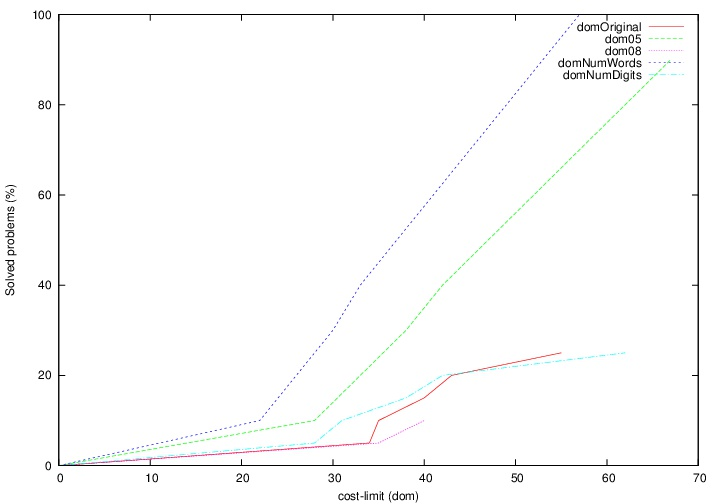
\includegraphics[width=6cm, height=6cm]{mff-or-05-08-word-digits-cost}
    \caption{MFF-or-05-08-word-digits-cost}
   \end{minipage}\hfill
   \begin {minipage}{0.48\textwidth}
     \centering
     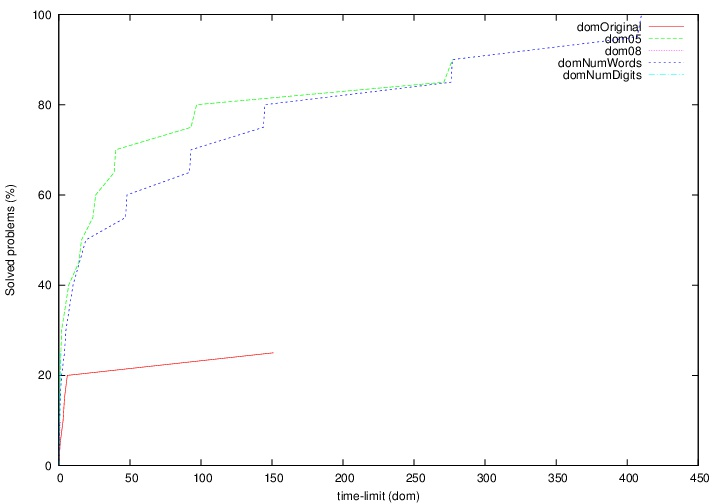
\includegraphics[width=6cm, height=6cm]{mff-or-05-08-word-digits-time}
    \caption{mff-or-05-08-word-digits-time}
   \end{minipage}
\end{figure}

\begin{figure}[!htb]
   \begin{minipage}{0.48\textwidth}
     \centering
     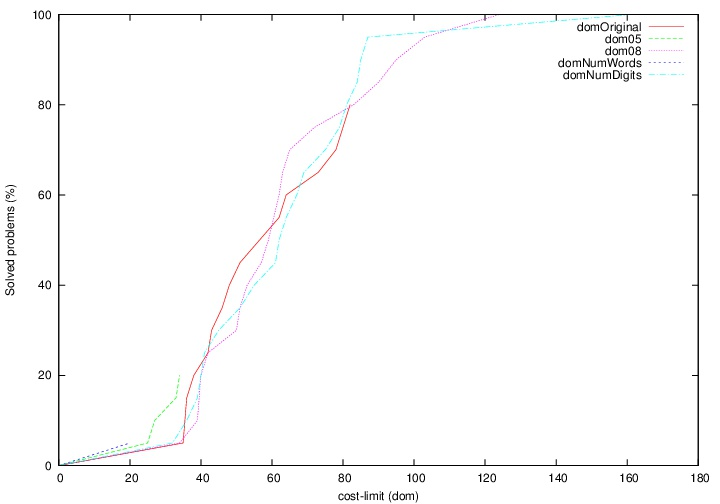
\includegraphics[width=6cm, height=6cm]{lpg-or-05-08-num-cost}
    \caption{lpg-or-05-08-num-cost}
   \end{minipage}\hfill
   \begin {minipage}{0.48\textwidth}
     \centering
     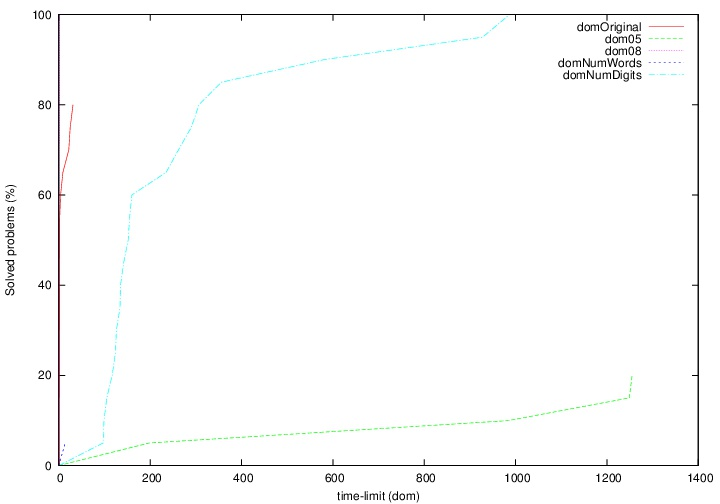
\includegraphics[width=6cm, height=6cm]{lpg-or-05-08-num-time}
    \caption{lpg-or-05-08-num-time}
   \end{minipage}
   
  \begin{minipage}{0.48\textwidth}
     \centering
     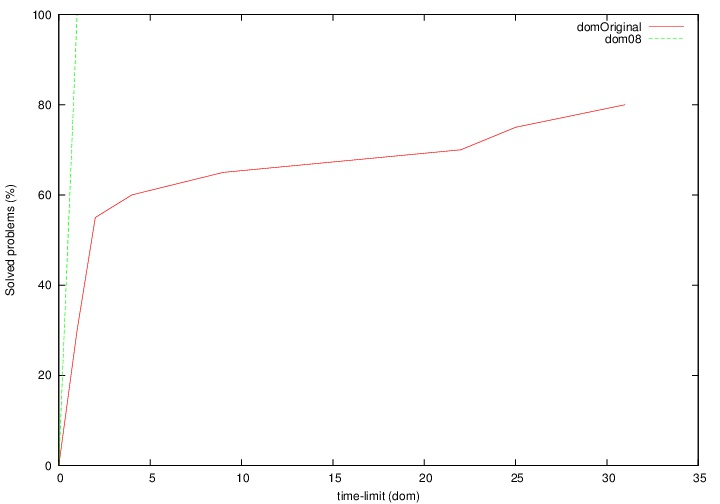
\includegraphics[width=6cm, height=6cm]{lpg-or-08-time}
    \caption{lpg-or-05-08-time}
   \end{minipage}\hfill
\end{figure}

\pagebreak

\paragraph{}
En la gráfica de resultados de tiempo de la ejecución con MFF, prácticamente no se ve el resultado de la versión numérica con dígitos generada automáticamente. Esto se debe a que está superpuesta con el principio de la versión 05. Al quedarse la gráfica en un valor de resolución de problemas del 25\% de los problemas de entrada, queda patente que esta versión comparada con el resto de versiones no es la mejor de las soluciones. Sin embargo, este resultado coincide con el porcentaje de problemas resueltos por la versión original requiriendo por otro lado mucho menos tiempo. Por otro lado, supera en el número de problemas resueltos y en un coste similar a la versión 08. A su vez, el coste de las soluciones obtenidas con la versión numérica con dígitos es similar al coste de la versión original, variando la versión con mayor coste entre estas dos versiones entre los distintos problemas resueltos.

\paragraph{}
Los mejores resultados obtenidos con el planificador MFF se obtienen con las versiones numérica con palabras y la versión 05, resolviendo más problemas y con menor coste con la versión automática numérica con palabras, pero requiriendo más tiempo que en la versión 05.

\paragraph{}
Respecto a la versión numérica con palabras generada automáticamente y la versión realizada manualmente (versión 05), se puede observar en los resultados obtenidos con el planificador MFF que en términos generales la versión generada automáticamente obtiene mejores resultados. En este caso, es difícil intentar desgranar los motivos subyacentes puesto que la versión automática genera bastantes nuevos predicados que son complicados de interpretar y la versión final que se genera tiene una estructura totalmente distinta de la que aparece en la versión manual.

\paragraph{}
Por otro lado, en las versiones numéricas con dígitos, los resultados son muy similares puesto que los problemas de entrada tienen una representación común y en lo único que varían los dominios es en uno de los operadores (toda la información referente a este cambio se puede encontrar en la sección de solución propuesta). En los resultados, se puede ver que con la versión automática se resuelven más problemas en la versión automática, teniendo esta un coste mayor pero obteniendo estas soluciones en un tiempo similar.

\paragraph{}
Respecto a los resultados de LPG, la versión automática numérica con palabras vuelve a resolver la totalidad de los problemas, al igual que también lo hace la versión numérica con palabras generada manualmente (la versión 08). Esto quiere decir que sin lugar a dudas la transformación automática para generar un dominio con palabras es beneficiosa para ambos planificadores.

\paragraph{}
Respecto a los costes para resolver los problemas, los menores costes se obtienen con la versión 08, que en su tramo de problemas iniciales se superpone con el coste de la versión original. En lo que concierne a los tiempos, la versión más rápida en la gráfica en la que aparecen representados los tiempos de las 5 versiones pudiera parecer que es la versión original. Sin embargo, en realidad la versión más rápida es la versión 08, como se puede ver en la gráfica adicional que se ha añadido incluyendo exclusivamente las gráficas de tiempo de la versión que aparenta ser la más rápida (la original) y la que realmente es significativamente más rápida (la versión 08). En la gráfica general de tiempos no se puede ver nítidamente el tiempo de la versión 08 debido a que como la diferencia de tiempos es tan grande respecto al resto de versiones, este tiempo está tan próximo a cero que es muy complicado ver estos tiempos en esta gráfica.

\subsubsection{Comparación del dominio12}

\paragraph{}
Este es un dominio por etapas en el que se ha intentado obtener la versión más óptima respecto a tanto el tiempo de búsqueda como al coste de obtención de las soluciones. Para crear este dominio, han sido necesarios añadir nuevos operadores que como se comentará a continuación han aumentado el coste de las soluciones.

\paragraph{}
Como este es el dominio que ha sido diseñado específicamente para ser el más óptimo de todos, no sólo se va a comparar el resultado con la versión original, sino que se va a comparar el coste de la solución de los problemas con el coste óptimo de la solución de cada uno de los problemas.

\paragraph{}
La solución óptima para cualquier problema de Childsnack (cuya lógica es en la que se ha basado esta versión del dominio) consiste en aprovechar que las bandejas tienen una capacidad infinita para únicamente utilizar una bandeja para la resolución del problema. A su vez, para cada niño que haya que servir hará falta: realizar un sándwich, cargarlo en la bandeja y servirlo. A su vez, considerando que la bandeja está en la cocina y todos los niños están en la misma localización, como mínimo será necesario el desplazamiento desde la cocina a la localización en la que estén todos los niños que haya que servir (salvo en el caso de que todos los niños estén en la cocina). Por otra, parte, en el peor de los casos, ninguna de las bandejas estará colocada inicialmente en la cocina (lo que supondrá el coste de una acción para desplazarla a la cocina para poder cargar los śandwiches) y cada niño estará en una posición distinta, por lo que a las acciones anteriores será necesario añadir una acción de desplazamiento de la bandeja por cada niño a servir. Por tanto, el número de pasos óptimo o coste para resolver cualquien problema de Childsnack queda definido por la siguiente fórmula: \\

$#niños\times3 \leq Coste \´optimo \leq niños\times4+1$

\paragraph{}
A partir de esta fórmula genérica, se puede acotar hasta saber directamente el coste exacto de la solución óptima si se cuenta con la información referente al número de localizaciones distintas en las que están los niños sin contar aquellos que puedan estar en la cocina ($a$) y si existe alguna bandeja en la cocina ($b$). Así, el coste exacto de la solución óptima para cualquier problema de Childsnack en su versión original es:

$Coste \´optimo = #niños\times3 + a + b$

\pagebreak

\begin{figure}[!htb]
   \begin{minipage}{0.48\textwidth}
     \centering
     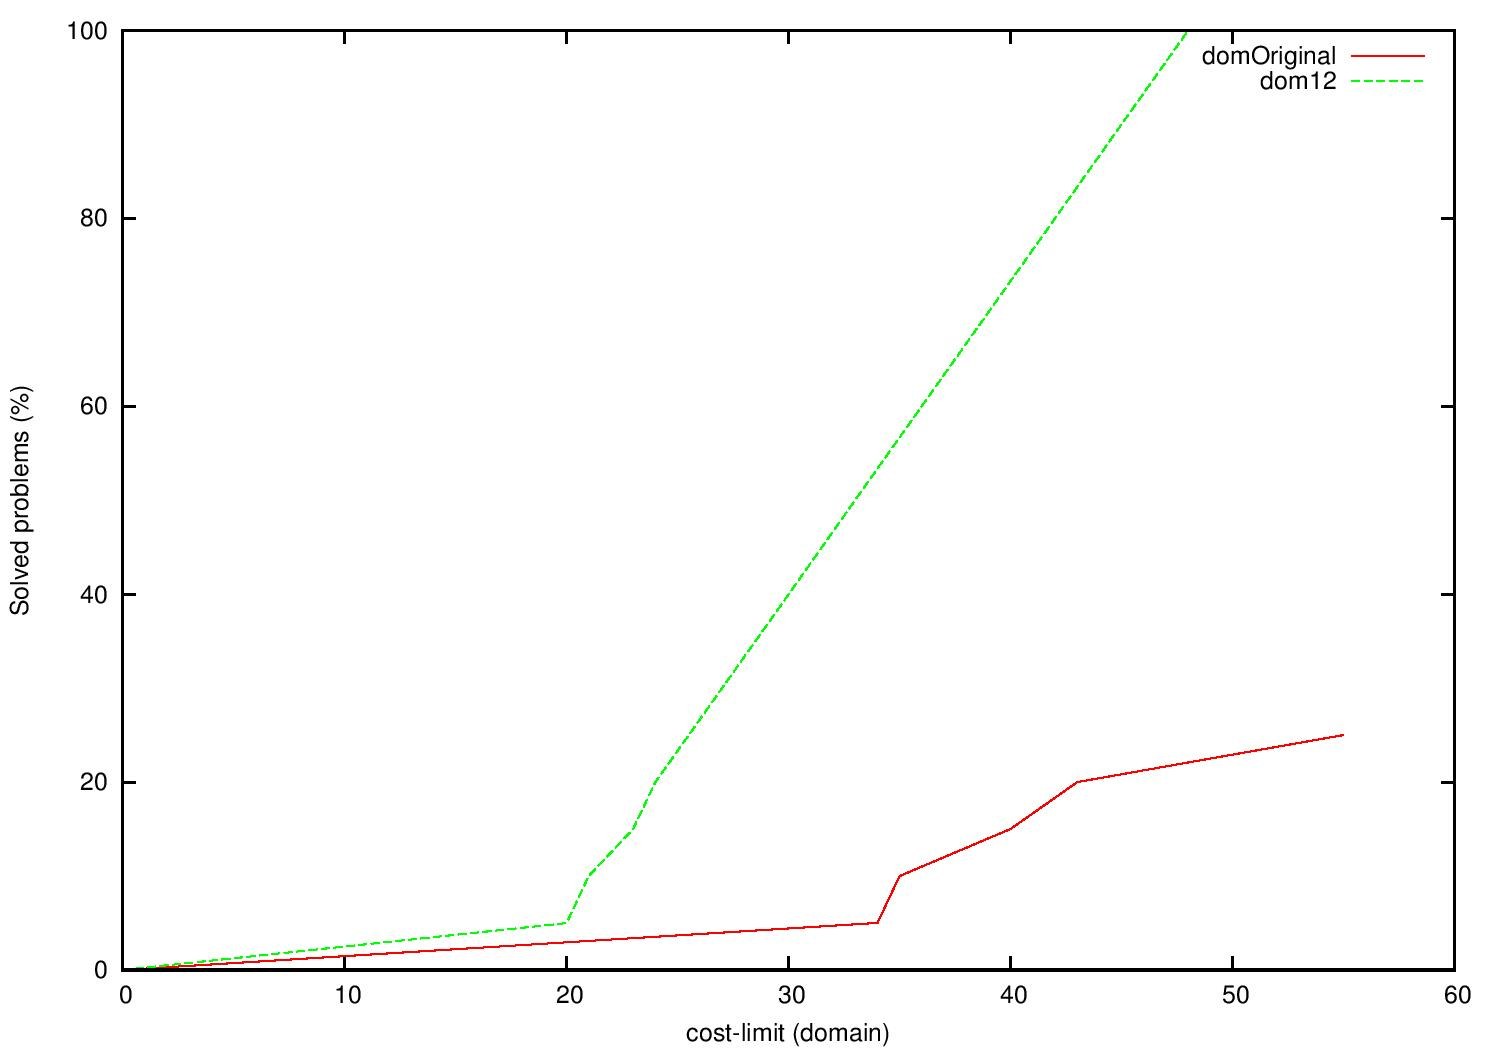
\includegraphics[width=6cm, height=6cm]{mff-or-12-cost}
    \caption{MFF-original-12-coste}
   \end{minipage}\hfill
   \begin {minipage}{0.48\textwidth}
     \centering
     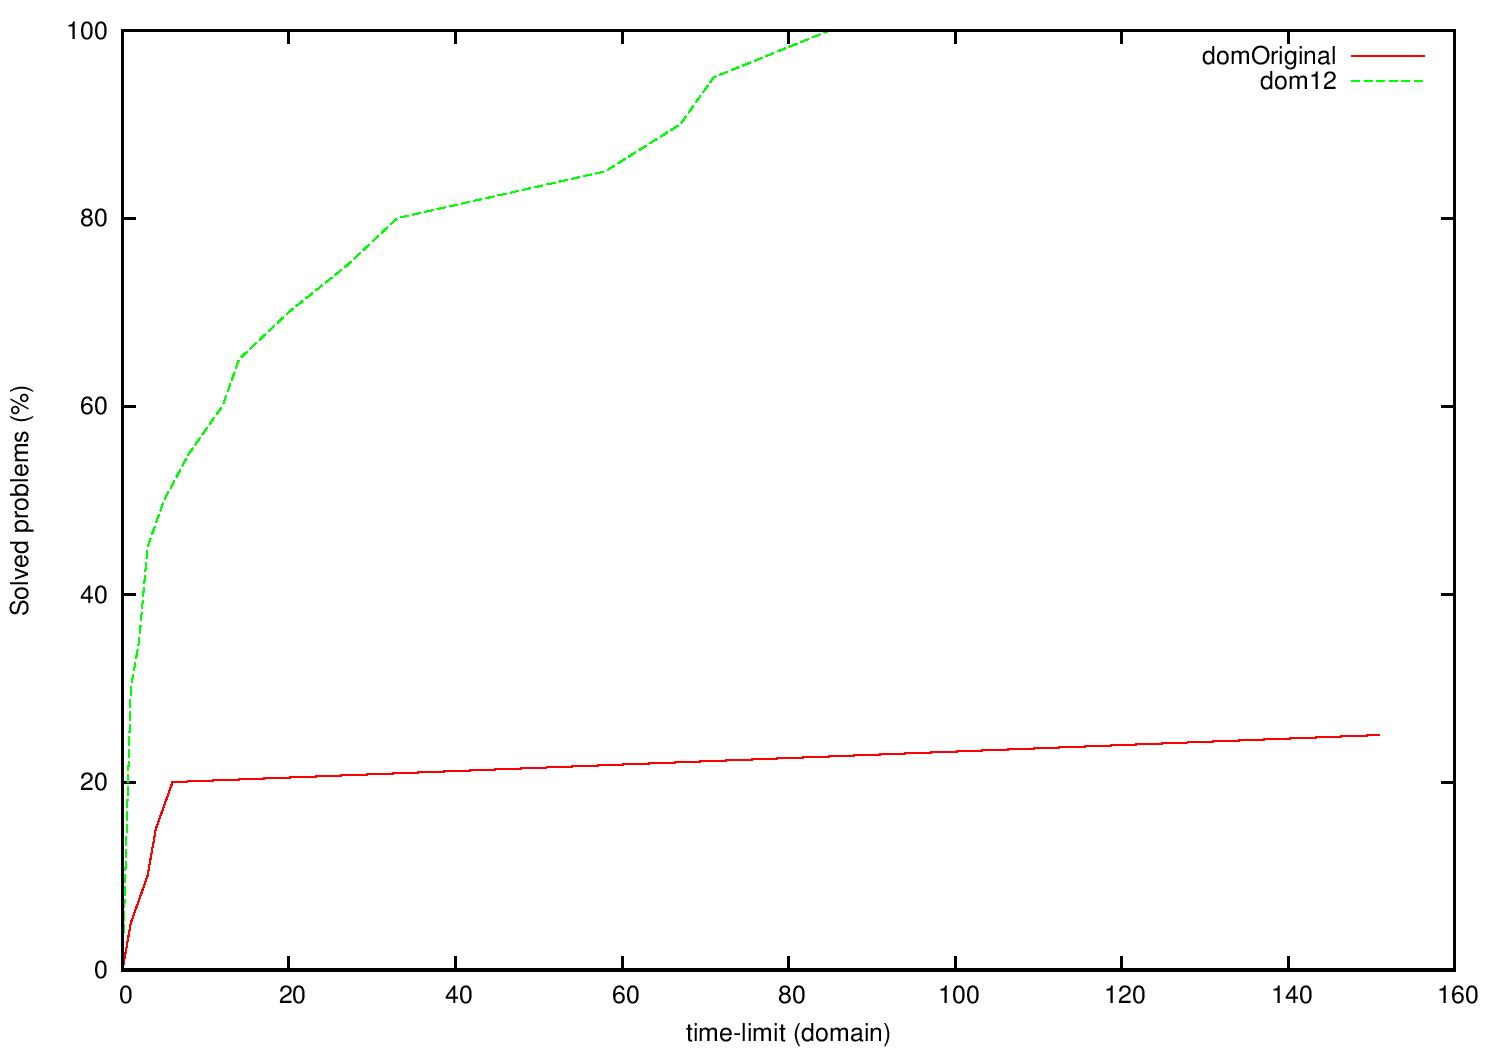
\includegraphics[width=6cm, height=6cm]{mff-or-12-time}
    \caption{MFF-original-12-tiempo}
   \end{minipage}
\end{figure}

\begin{figure}[!htb]
   \begin{minipage}{0.48\textwidth}
     \centering
     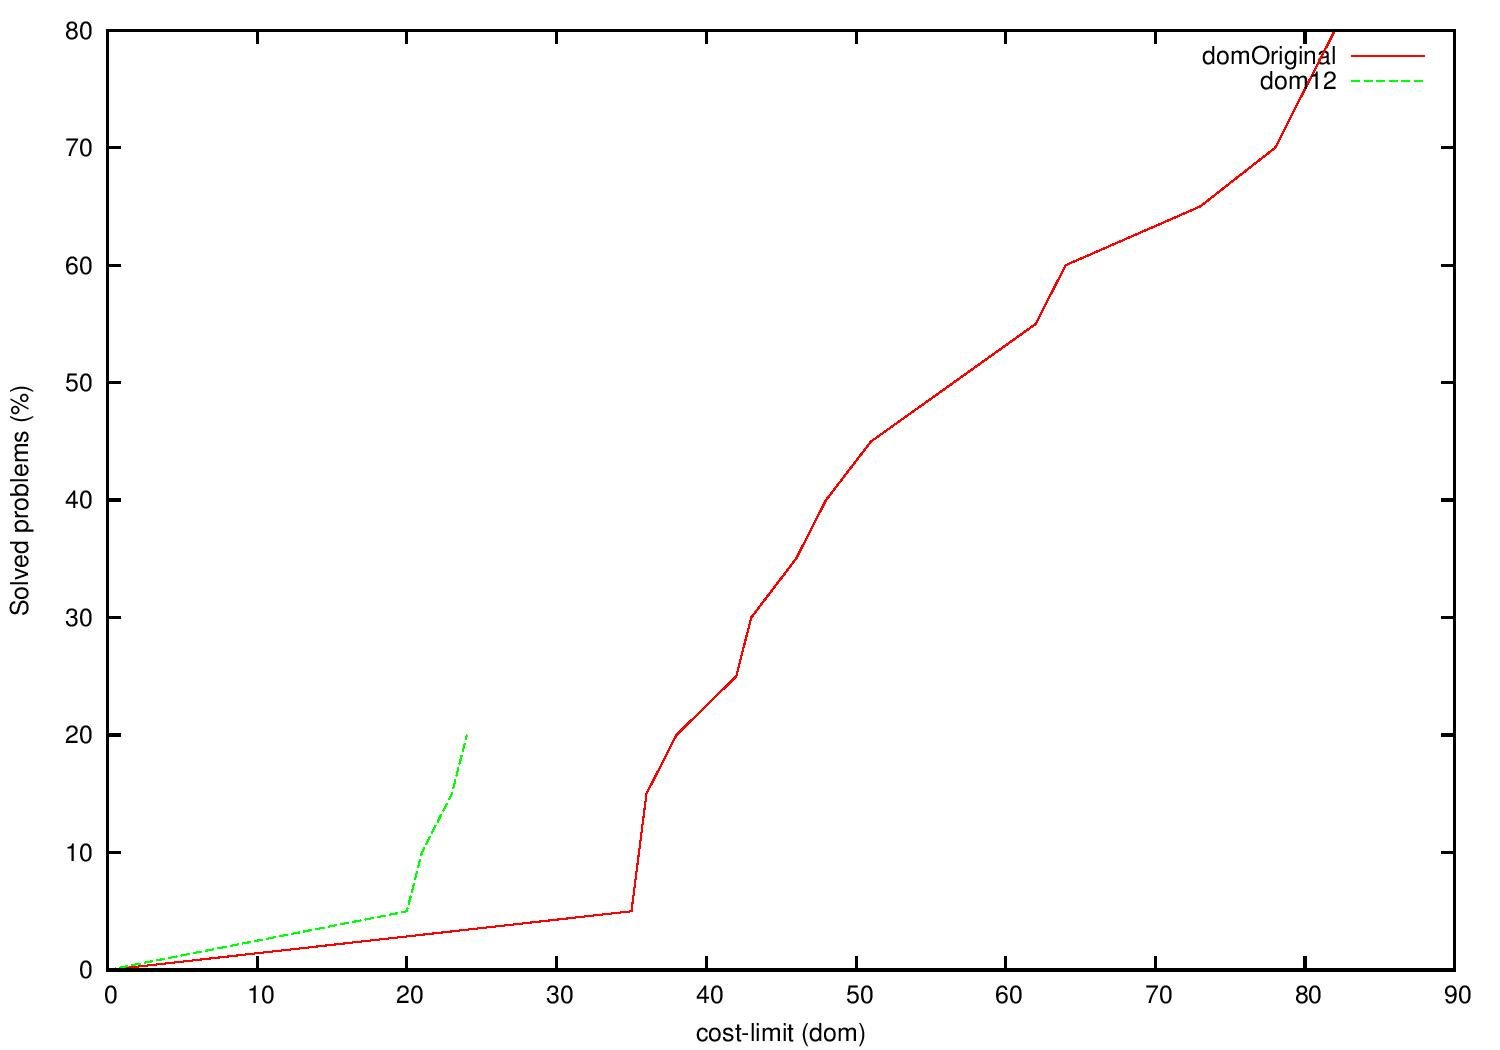
\includegraphics[width=6cm, height=6cm]{lpg-or-12-cost}
    \caption{LPG-original-12-coste}
   \end{minipage}\hfill
   \begin {minipage}{0.48\textwidth}
     \centering
     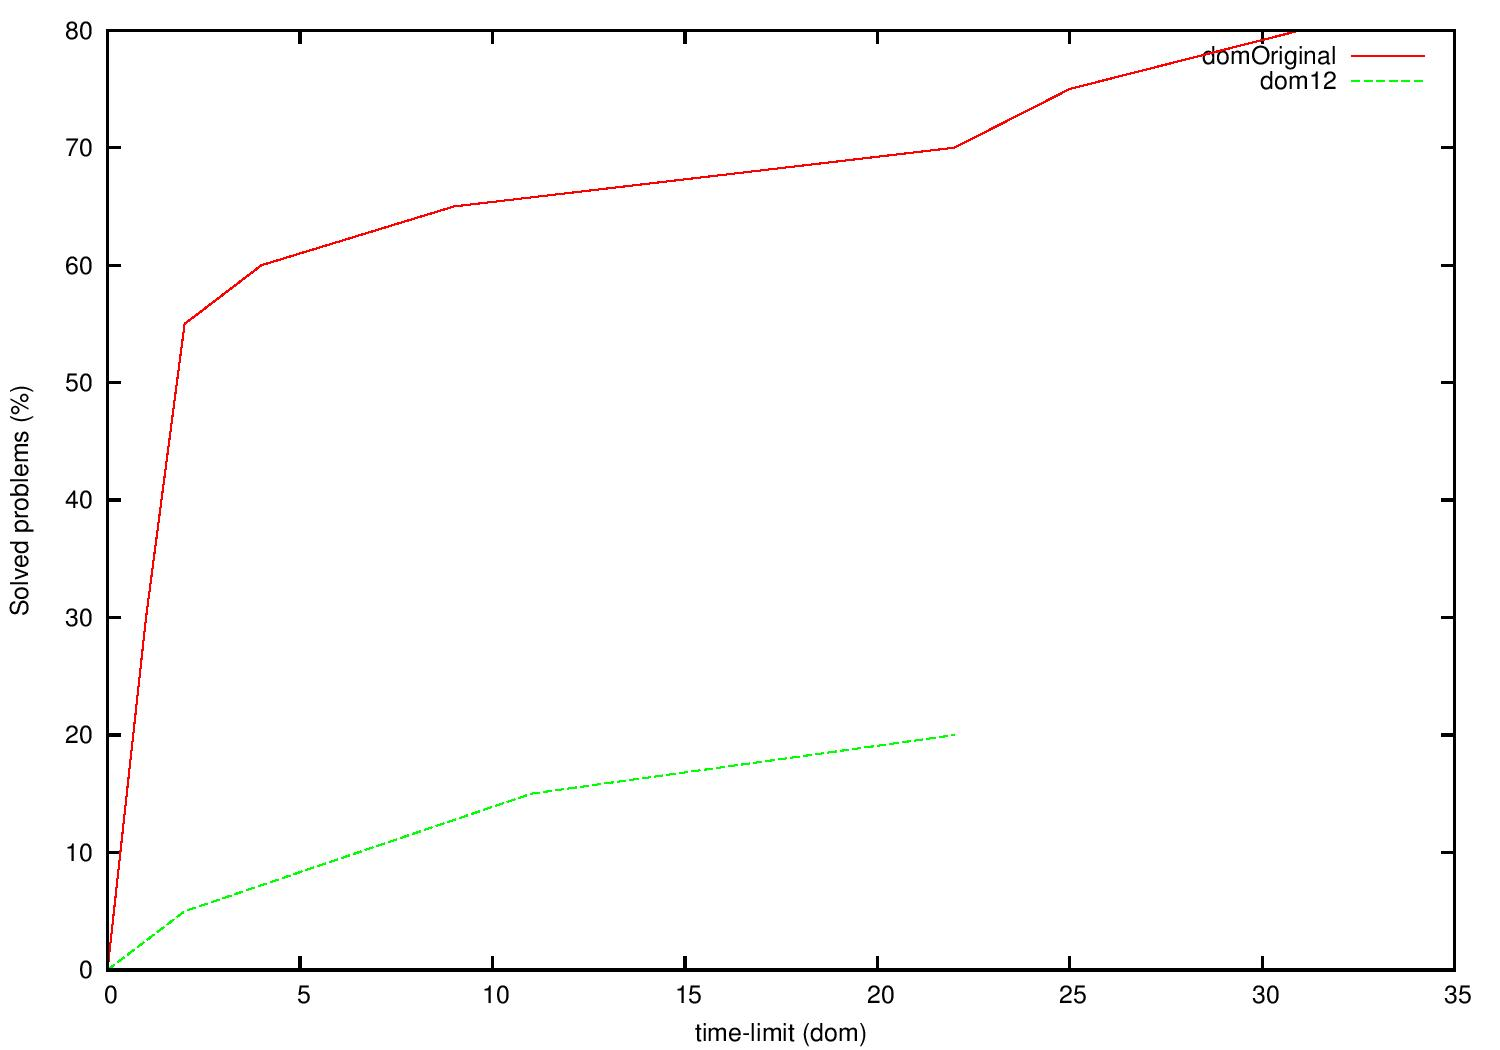
\includegraphics[width=6cm, height=6cm]{lpg-or-12-time}
    \caption{LPG-original-12-tiempo}
   \end{minipage}
\end{figure}

\begin{table}[H]
\centering
\caption{Coste óptimo y coste de MFF}
\label{my-label}
\begin{tabular}{|c|c|c|}
\hline
\textbf{Problema} & \textbf{Coste óptimo} & \textbf{Coste MFF} \\ \hline
01-2              & 21                    & \textbf{21}        \\ \hline
01                & 20                    & \textbf{20}        \\ \hline
02-2              & 24                    & \textbf{24}        \\ \hline
02                & 22                    & 23                 \\ \hline
03-2              & 27                    & \textbf{27}        \\ \hline
03                & 27                    & \textbf{27}        \\ \hline
04-2              & 30                    & \textbf{30}        \\ \hline
04                & 30                    & \textbf{30}        \\ \hline
05-2              & 33                    & \textbf{33}        \\ \hline
05                & 33                    & \textbf{33}        \\ \hline
06-2              & 36                    & \textbf{36}        \\ \hline
06                & 36                    & \textbf{36}        \\ \hline
07-2              & 39                    & \textbf{39}        \\ \hline
07                & 39                    & \textbf{39}        \\ \hline
08-2              & 39                    & 42                 \\ \hline
08                & 39                    & 42                 \\ \hline
09-2              & 45                    & \textbf{45}        \\ \hline
09                & 45                    & \textbf{45}        \\ \hline
10-2              & 48                    & \textbf{48}        \\ \hline
10                & 48                    & \textbf{48}        \\ \hline
\end{tabular}
\end{table}

\paragraph{}
Como se puede ver en las gráficas, vuelve a haber una gran diferencia entre las gráficas obtenidas con MFF y con LPG-td. En el caso de MFF, se puede ver que esta modificación mejora muy significativamente tanto los tiempos de búsqueda como la calidad de las soluciones encontradas, hasta el punto de que como se puede observar en la tabla superior, en 17 de los 20 problemas originales el coste de la solución obtenida es el mismo que el menor que se podría obtener en cualquier versión que se hiciese de este problema, lo que convierte a esta versión en la mejor de todas las creadas.

\paragraph{}
Por contra, se puede observar que los resultados obtenidos utilizando el planificador LPG-td son bastante peores que los obtenidos por la versión original en coste, tiempo de resolución y porcentaje de problemas resueltos.

\end{document}